\documentclass[a4, 12pt, landscape]{article}

\usepackage{hyperref}
\usepackage[danish]{babel}
\usepackage[T1]{fontenc}
\usepackage[utf8]{inputenc}
\usepackage{listings}
\usepackage{color}
\definecolor{bluekeywords}{rgb}{0.13,0.13,1}
\definecolor{greencomments}{rgb}{0,0.5,0}
\definecolor{redstrings}{rgb}{0.9,0,0}
\usepackage{subfigure}
\usepackage{graphicx}
\usepackage{amsmath}
\usepackage{amssymb}
\usepackage{tikz}

\usepackage[simplified]{pgf-umlcd}

\usetikzlibrary{shapes.geometric, arrows}

\tikzstyle{startstop} = [rectangle, rounded corners, minimum width=3cm, minimum height=1cm,text centered, draw=black, fill=red!30]
\tikzstyle{io} = [trapezium, trapezium left angle=70, trapezium right angle=110, minimum width=3cm, minimum height=1cm, text centered, draw=black, fill=blue!30]
\tikzstyle{process} = [rectangle, minimum width=3cm, minimum height=1cm, text centered, text width=3cm, draw=black, fill=orange!30]
\tikzstyle{decision} = [diamond, minimum width=3cm, minimum height=1cm, text centered, draw=black, fill=green!30]
\tikzstyle{arrow} = [thick,->,>=stealth]


\lstset{language=[Sharp]C,
  showspaces=false,
  showtabs=false,
  breaklines=true,
  showstringspaces=false,
  breakatwhitespace=true,
  escapeinside={(*@}{@*)},
  escapeinside={\%}{)},
  commentstyle=\color{greencomments},
  keywordstyle=\color{bluekeywords},
  stringstyle=\color{redstrings},
  basicstyle=\ttfamily,
  captionpos=b,
  frame=single,
  framesep=2pt,
  tabsize=3,
  numbers=left,
  stepnumber=1
}



\title{Indledende Diagram}

\author{Uffe Thorsen, \href{mailto:utho@zbc.dk}{\texttt{utho@zbc.dk}}}

\pagestyle{empty}

\begin{document}

\thispagestyle{empty}
\hspace{-3cm}
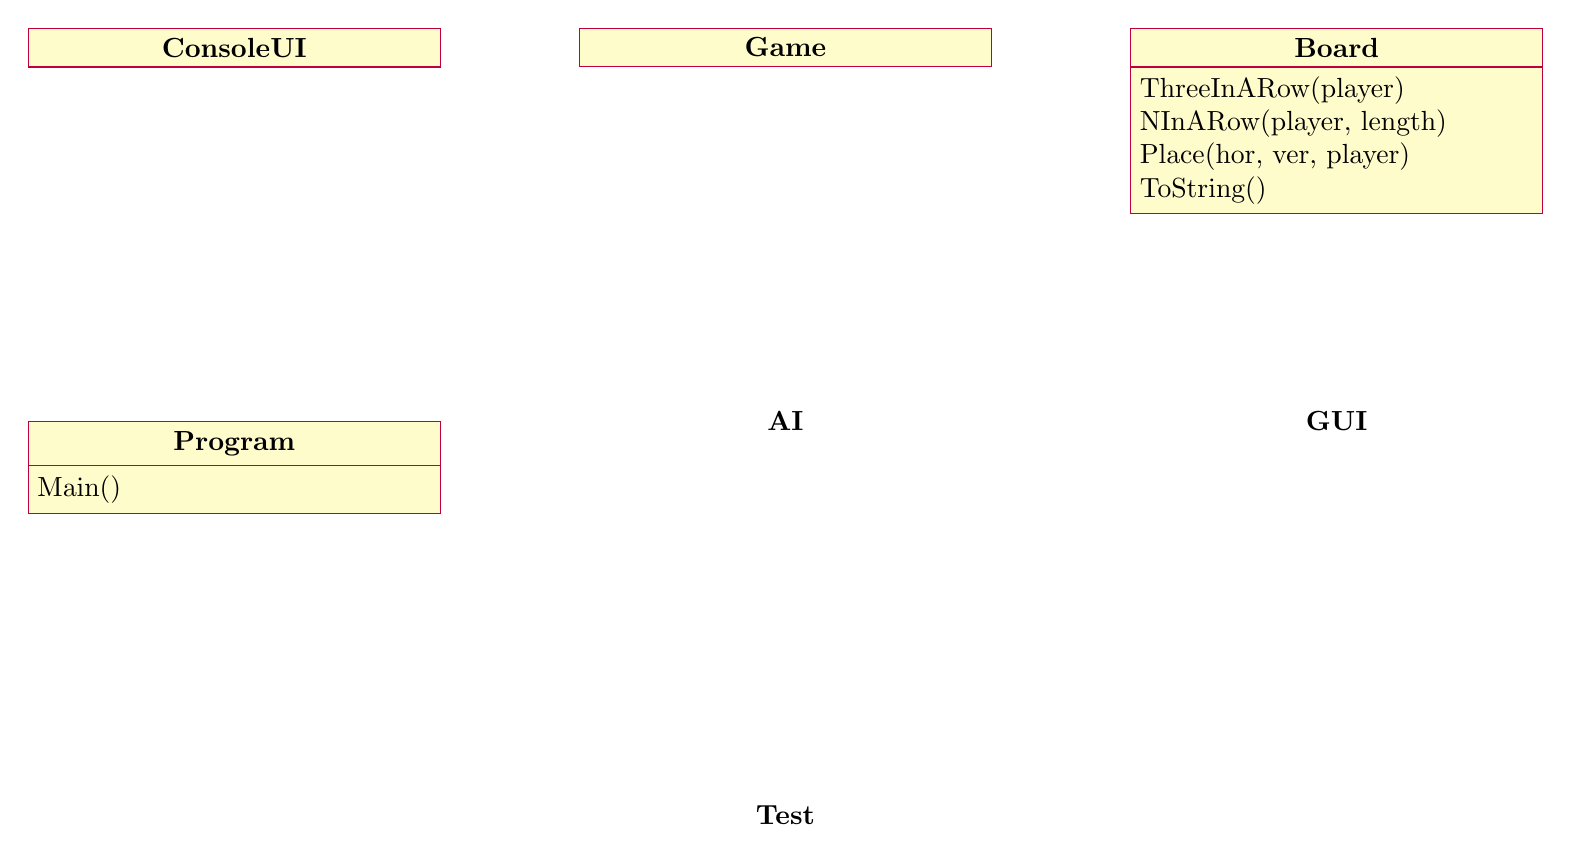
\begin{tikzpicture}

%class Program
\begin{class}[text width=5cm]{Program}{0,-10}
%	\attribute{game}
	\operation{Main()}
\end{class}

%class ConsoleUI
\begin{class}[text width=5cm]{ConsoleUI}{0,-5}

\end{class}

%class Game
\begin{class}[text width=5cm]{Game}{7,-5}

\end{class}

%class Board
\begin{class}[text width=5cm]{Board}{14,-5}
	\operation{ThreeInARow(player)}
	\operation{NInARow(player, length)}
	\operation{Place(hor, ver, player)}
	\operation{ToString()}
\end{class}


%AI
\node (ai) at (7,-10) {\textbf{AI}};

%GrafiskUI
\node (gui) at (14, -10) {\textbf{GUI}};

%Test
\node (test) at (7, -15) {\textbf{Test}};

\end{tikzpicture}




\newpage

\hspace{-3cm}
\begin{tabular}{c|l|l}
\textbf{class/enhed} & \textbf{Ansvar} & \textbf{Ansvarlig}\\
\hline
Program & At starte det hele op. & \\
ConsoleUI & Håndter I/O over konsollen. & Tobias\\
Game & Hvilken spiller der har tur. Om nogen har vundet. & Birk\\
Board & Placering af brikker. Om der er 3 på stribe. & Daniel\\
\end{tabular}

\vfill{}

\section*{Andre roller:}

\begin{tabular}{c|l}
\textbf{Rolle} & \textbf{Person}\\
\hline
Project owner & Uffe\\
Sekretær & Uffe\\
Projektledere & Knigge, Mathias \\
\end{tabular}


\vfill{}

\end{document}